\documentclass[a4paper,11pt]{article}
\usepackage{jheppub} % for details on the use of the package, please see the JINST-author-manual
\usepackage{lineno}
\usepackage{amsmath,amsthm,amsfonts,amssymb,amscd,physics,cancel,mathtools}
\usepackage{tcolorbox}
\usepackage{marginnote,tensor}
%~~~~~~~~~ Document setup
% \usepackage[spanish]{babel} % English formatting
\usepackage[utf8]{inputenc} % Standard encoding
% \usepackage[a4paper,left=3cm,bottom=3cm]{geometry} % Page formatting
\usepackage{indentfirst} % Indents the first paragraph
\usepackage{amsmath} % Maths type package
\usepackage{bm} % Bold font maths
\usepackage{graphicx} % Advanced graphics package
\usepackage[export]{adjustbox} 
\usepackage{pdflscape} % Make pages landscape
\usepackage{fancyhdr} % Fancy headers
% \usepackage[colorlinks=true,citecolor=blue,urlcolor=blue,linkcolor=black]{hyperref} % Link colours
%\usepackage{natbib} % Bibliography
% \usepackage{flafter} % Reference any 'float'
% \usepackage[framemethod=tikz]{mdframed} % Box off stuff
\usepackage{color} % Colour support
\usepackage{wrapfig} % Text flowing around figures
\usepackage{lipsum} % Generates meaningless text
\usepackage{xcolor}
% \usepackage{biblatex}
% \addbibresource{sample.bib}
\hypersetup{colorlinks=true, linkcolor=blue}

\newtheorem{ej}{Example}[section]
\newtheorem{sol}{Solution}[section]
\newtheorem{dem}{Proof}[section]




% \arxivnumber{1234.56789} % if you have one

\title{\boldmath Teoría Clásica de Campos}

% Collaborations

%% [A] If main author
%% \collaboration{\includegraphics[height=17mm]{collabroation-logo}\\[6pt]
%%  XXX collaboration}

%% or
%% [B] If "on behalf of"
%% \collaboration[c]{on behalf of XXX collaboration}


% Authors
% The "\note" macro will give a warning: "Ignoring empty anchor...", you can safely ignore it.

%% [A] simple case: 2 authors, same institution
%% \author[1]{A. Uthor\note{Corresponding author.}}
%% \author{and A. Nother Author}
%% \affiliation{Institution,\\Address, Country}

%% or, e.g.
%% [B] more complex case: 4 authors, 3 institutions, 2 footnotes
%% \author[a,b]{F. Irst,\note{Now at another university}}
%% \author[c]{S. Econd,}
%% \author[a,2]{T. Hird\note{Also at Some University.}}
%% \author[c,2]{and Fourth}
%% \affiliation[a]{Institution_1,\\Address, Country}
%% \affiliation[b]{Institution_2,\\Address, Country}
%% \affiliation[c]{Institution_3,\\Address, Country}

\author{Borja Diez}
\affiliation{Universidad Arturo Prat}
% \affiliation{Another University,\\
% different-address, Country}

% E-mail addresses: only for the corresponding author
\emailAdd{borjadiez1014@gmail.com}

\abstract{Abstract...}





\begin{document}
\maketitle
\flushbottom

\part{Mecánica Clásica}
\section{Clase 1}
\subsection{Mecánica de Newton}
Posición, velocidad, aceleración, fuerza.

Si consideramos un sistema de partículas de masa $m$
\begin{equation}
  \vec{p}_\alpha =m_\alpha \vec{\dot{x}}_\alpha,\qquad \vec{p}=\sum_\alpha \vec{p}_\alpha,\qquad \alpha=1,...,k
\end{equation}
\begin{equation}
  T=\frac{1}{2}\sum_\alpha m_\alpha \vec{\dot{x}}^2,\qquad \vec{L}=\sum_\alpha \vec{x}_\alpha\times \vec{p}_\alpha
\end{equation}
Newton estableció que a dinámica de un sistema mecánico queda	determinada por tres leyes fundamentales:
\begin{itemize}
	\item \textbf{Primera ley del movimiento:} Todo cuerpo en reposo permanecerá en reposo o en movimiento rectilíneo uniforme (MRU), a menos que una fuerza externa actúe sobre él.
	\item \textbf{Primera ley del movimiento:} Un cuerpo cambia su estado de movimiento si una fuerza actúa sobre él
	\begin{equation}
  \vec{F}=m\vec{a}
\end{equation}

\item \textbf{Tercera ley del movimiento:} A cada acción le corresponde una reacción paralela y opuesta.
\end{itemize}

Estas lees sólo son válidas en un sistema de referencia inercial (SRI). Dos SRI están relacionados por medio de una transformación de Galileo.

\begin{figure}[h!]
	\centering
	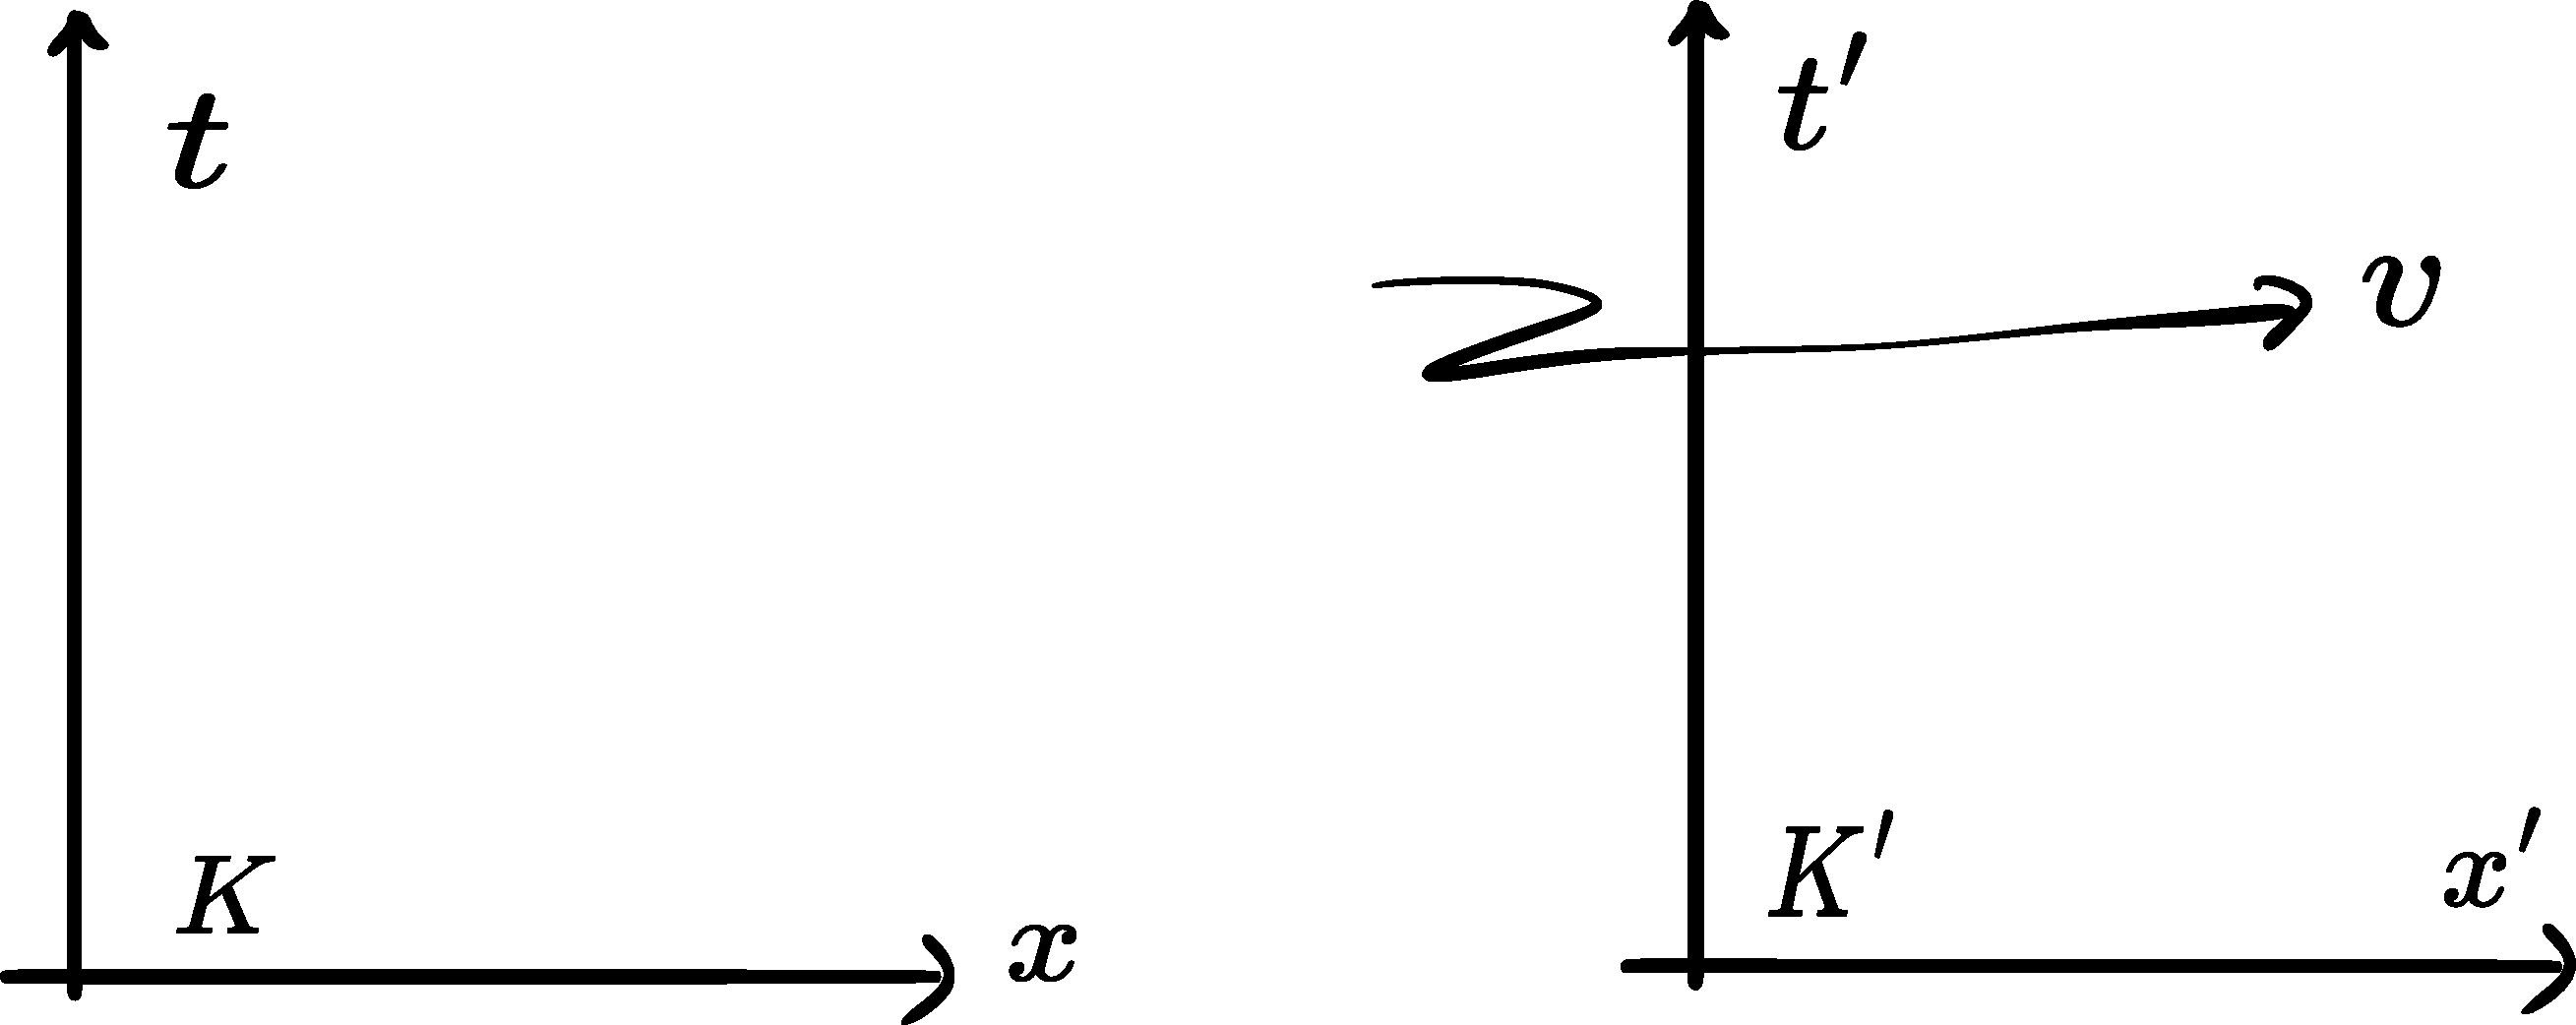
\includegraphics[scale=0.2]{fig/Galileo.pdf}
\end{figure}

\begin{align}
  x'&=x-vt\\
  t'&=t
\end{align}

Además
\begin{align}
  \vec{F}_\a &=m\ddot{\vec{x}}
\end{align}
\begin{equation}
	\implies m\ddot{\vec{x}}_\a =\dv{t}(m\dot{\vec{x}}_\a )=\dv{t}\vec{p}_\a =\dot{\vec{p}}_\a 
\end{equation}
Si las fuerzas son conservativas, se tiene
\begin{equation}
  \vec{F}_\a =-\vec{\nabla} V_\a 
\end{equation}
\begin{equation}
  \implies \boxed{\vec{\dot{p}}_\a +\vec{\nabla}V_\a =0}
\end{equation}

\subsection{Mecánica de Lagrange}
Es basada en la llamada función de Lagrange, definida como
\begin{equation}
  L(\vec{x}_\a ,\dot{\vec{x}}_\a ,t)=T(\dot{\vec{x}}_\a ,t)-V(\vec{x}_\a ,t)
\end{equation}
Lagrange introdujo el concepto de coordenada generalizada
\begin{equation}
  q_i,\quad i=1,2,...,f
\end{equation}
donde $f$ son los grados de libertad del sistema. De esta manera, se define la derivada de Euler-Lagrange como
\begin{equation}
  [L]_i=\EL=0
\end{equation}
Así, las soluciones a estas ecuaciones describen la dinámica del sistema en un espacio $f$-dimensional de coordenadas $q_i,q_2,...,q_f$.

\underline{\textbf{Nota}}: La energía cinética debe ser una función homogénea de grados dos
\begin{equation}
  T=\sum_{i,k} a_{ik}\qd_i\qd_k
\end{equation}

Notemos que una función de Lagrange dada por
\begin{equation}
  L'=L+\dv{t}B(q,t)
\end{equation}
conduce a las mismas ecuaciones del movimiento.

La libertad en la elección de coordenadas generalizadas implica que las ecuaciones de movimiento de Euler-Lagrange son \textit{estructuralmente invariantes} bajo una transofrmación de coordenadas generalizadas, es decir, bajo
\begin{equation}
  q_i\to q'_i=q'_i(q_l)\implies \qd '_i=\pdv{q'_i}{q_l}\qd_l
\end{equation}
\begin{equation}
  \pdv{\qd'_i}{\qd _l}=\pdv{q'_i}{q_l}
\end{equation}
Definiendo 
\begin{equation}
  \varphi(q_l)=\pdv{q'_i}{q_l}
\end{equation}
se tiene
\begin{equation}
  \dv{t}\varphi(q_l)=\pdv{\varphi}{q_l}\dot{q}_l
\end{equation}
luego
\begin{equation}
  \dv{t}\pdv{q'_i}{q_l}=\pdv{q_k}\left(\pdv{q'_i}{q_l}\right)\qd_k
\end{equation}
\begin{equation}\label{1.1}
  \implies \boxed{\dv{t}\pdv{q'_i}{q_l}=\pdv{q'_i}{q_k}{q_l}\qd_k}
\end{equation}
Dado que
\begin{equation}
  \qd'_i=\pdv{q'_i}{q_l}\qd_i
\end{equation}
\begin{equation}\label{1.2}
  \pdv{\qd_i}{q_l}=\pdv{q_l}\left(\pdv{\qd_i}{q_k}\qd_k\right)=\pdv{\qd_i}{q_l}{q_k}\qd_k+\cancelto{0}{\pdv{\qd_i}{q_k}\pdv{\qd_k}{q_l}}
\end{equation}
\begin{equation}
  \implies \boxed{\dv{t}\pdv{q'_i}{q_l}=\pdv{\qd_i}{q_l}}
\end{equation}
Dado que $L'(q',\qd',t)=L(q,\qd,t)$, calculemos
\begin{equation}
  \dv{t}\pdv{L'}{\qd'_k}
\end{equation}























\subsection{Acerca de la matriz Hessiana de las ecuaciones de Euler-Lagrange}
\begin{equation}
  \dv{t}\pdv{L'}{\dot{q}'_k}=\pdv{L'}{q'_k}-[L]_k\pdv{q_l}{\dot{q}_k}
\end{equation}
\begin{equation}
  \Rightarrow \pdv{L'}{q'_k}=\dv{t}\pdv{L'}{\dot{q}_k}=[L]_l\pdv	{q_l}{q'_k}
\end{equation}
\begin{equation}
\boxed{[L']_k=[L]_l\pdv{q_l}{q'_k}}
\end{equation}
La derivada de Euler-Lagrange transforma como un vector covariante bajo una transformación de coordenadas
\begin{equation}
  \mbox{Si }[L]_l=0 \Rightarrow [L']_k=0
\end{equation}



\section{Clase 2}
\begin{enumerate}
	\item Las ecuaciones de Newton son invariantes en forma bajo las transformaciones de Galileo.
	\item Las ecuaciones de Newton sn ecuaciones de segundo orden en $\vb*{x}_\alpha$. Es bueno recalcar que \textit{todas las ecuaciones dinámicas de la física fundamental son de segundo orden}. Las ecuaciones de orden mayor al segundo, tienden a tener inestabilidades \cite{Ostrogradsky:1850fid}.
	\item Si $L=L(q_i,\dot{q}_i,t)$ es la función de Lagrange para un sistema mecánico, entonces la dinámica del sistema es gobernada por las ecuaciones de Euler-Lagrange,
	\begin{equation}\label{eqs EL}
  [L]_i=\pdv{L}{q_i}-\dv{t}\pdv{L}{\dot{q}_i}=0
\end{equation}
Estas ecuaciones no cambian si la función de Lagrange es modificada a la forma
\begin{equation}
  \tilde{L}=L+\dv{t}B(q,t)
\end{equation}
con $L=L(q_i,\dot{q}_i,t)$ y $\bar{L}=\bar{L}(q_i,\dot{q}_i,t)$
\item La libertad en la elección de las coordenadas generalizadas implica que las ecuaciones de Euler-Lagrange son estructuralmente invariantes bajo un cambio de coordenadas:
\begin{equation}\label{2.1}
  q_i\to q'_i=q'_i(q_l)
\end{equation}
lo cual implica que
\begin{equation}
  \boxed{[L']_k=[L]_l\pdv{q_l}{q'_k}}
\end{equation}
que muestra que la derivada de Euler transforma como un vector covariante bajo la transformación \ref{2.1}
\end{enumerate}
\begin{equation}
  \mbox{Si }[L]_l=0 \Rightarrow [L']_k=0.
\end{equation}

Es importante recalcar que la invariancia estructural es distinto a la invariancia en forma (covariancia).

\textit{Todos los observadores observan la misma forma de las ecuaciones de los modelos de la naturaleza.}

\begin{ej}
	La ecuación de Newton en el SRI K toma la forma $\vb*{F}=m\vb*{a}$ mientras que en el SRI $K'$ toma la forma $\vb*{F'}=m'\vb*{a}'$.
\end{ej}
\begin{ej}
	Las ecuaciones de Maxwell tendrán la misma forma en todos los SRI.
\end{ej}

Notemos son embargo, que en la mecánica de Newton las transformaciones son las transformaciones de Galileo y que en la electrodinámica de Maxwell son las transformaciones de Lorentz.

La covariancia de las ecuaciones del movimiento bajo una transformación de coordenadas es la propiedad que define una \textbf{simetría de Lie}.

\subsection{Acerca de la matriz Hessiana}
Una característica básica de las ecuaciones de Newton $m\ddot{\vb*{r}}=\vb*{F}(\vb*{r},\dot{\vb*{r}},t)$ es que es posible expresar la aceleración $\ddot{\vb*{r}}$ en función de la posición $\vb*{r}$, de la velocidad $\dot{\vb*{r}}$ y de $t$,
\begin{equation}
  \ddot{\vb*{r}}(t)=\frac{1}{m}\vb*{F}(\vb*{r},\dot{\vb*{r}}(t))
\end{equation}
Esta es una formulación vectorial de la mecánica  es basada en el concepto d partícula material. Esto llevó a pensar que la naturaleza podría no ser contínua, sino que podría ser atómica (cuántica). Esto condujo a la formulación escalar de la mecánica representado de la introducción del concepto de energía.

La formulación de Lagrange y de Hamilton fue el resultado de esta búsqueda. Sin embargo, de las ecuaciones de Euler-Lagrange \eqref{eqs EL} no es evidente cómo expresar la aceleración $\ddot{q}(t)$ en función de $q(t), \dot{q}(t)$ y $t$.

Consideremos
\begin{equation}
	\dv{t}\pdv{L}{\dot{q}_n},\qquad L=L(q_n,\dot{q}_n,t)
\end{equation}
notemos que
\begin{equation}
  \dv{t}\pdv{L}{\dot{q}_n}=\pdv{L}{\dot{q}_n}{\dot{q}_m}\ddot{q}^m+\pdv{L}{\dot{q}_n}{q_m}\dot{q}^m
\end{equation}
luego
\begin{equation}
  [L]_n=\pdv{L}{q_n}-\pdv{L}{\dot{q}_n}{q_m}\dot{q}^m-\pdv{L}{\dot{q}_n}{\dot{q}_m}\ddot{q}^m=0
\end{equation}
así
\begin{equation}
  \boxed{\left(\pdv{L}{\dot{q}_n}{\dot{q}_m}\right)\ddot{q}^m=\pdv{L}{q_n}-\pdv{L}{\dot{q}_n}{q_m}\dot{q}^m}
\end{equation}
Notemos que para poder expresar $\ddot{q}$ como función de $q$ y $\dot{q}$ es necesario que la matriz $W_{nm}=\pdv*{L}{\dot{q}_n}{\dot{q}_m}$ sea invertible, es decir, $\det W_{nm}\neq 0$.

Llamando 
\begin{equation}
V_n=\pdv{L}{q_n}-\pdv{L}{\dot{q}_n}{q_m}{\dot{q}^m}
\end{equation}
tenemos
\begin{equation}\label{2.2}
  W_{nm}\ddot{q}^{m}-V_n=0
\end{equation}
Si $\det W_{nm}\neq 0$ entonces existe una matriz inversa $W^{kn}\equiv (W_{kn})^{-1}$ tal que $W^{kn}W_{nm}=\delta ^k_m$. Luego, multiplicando \eqref{2.2} por $W^{km}$, tenemos
\begin{align}
 & W^{kn}W_{nm}\ddot{q}^m-W^{kn}V_n=0\\
  \Rightarrow \ & \ddot{q}^k=W^{kn}V_n=F(q,\dot{q},t)
\end{align}
En la física fundamental, las teorías de gauge tales como la teoría electromagnética o las toerías de Yang-Mills (teoría electrodébil, cromonodinámica cuántica), las correspondientes funciones de Lagrange tienen sus matrices Hessianas singulares, es decir, $\det W_{nm}\neq 0$.

\subsection{Formalismo de Hamilton}
Consiste en pasarse de las coordenadas $\{q_i,\dot{q}_i,t\}$ a $\{q_i,p_i,t\}$, donde
\begin{equation}\label{2.3}
  p_i=\pdv{L}{\dot{q}_i}=f_i(q_i,\dot{q}_i,t)
\end{equation}
es el momentum generalizado.

Para escribir explícitamente la función de Hamilton es necesario expresar por medio de \eqref{2.3} $\dot{q}_i=\bar{f}(q_i,p_i)$. Esto implica que la función $f_i$ sea invertible,
\begin{equation}
  \dot{q}_n\to p_n=f_n(q_m,\dot{q}_m,t)
\end{equation}
es decir, tenemos una transformación de coordenadas. Esta transformación tiene como matriz Jacobiana a 
\begin{equation}
  J_{nm}=\pdv{f_n}{\dot{q}_m}=\pdv{p_n}{\dot{q}_m}=\pdv{\dot{q}_m}\left(\pdv{L}{\dot{q}_n}\right)
\end{equation}
esto es
\begin{equation}
  \boxed{J_{nm}=\pdv{L}{\dot{q}_n}{\dot{q}_m}\equiv W_{nm}}
\end{equation}

Para clarificar esto calculemos $\dd p_n$ recordando que $p_n=f_n(q_m,\dot{q}_m,t)$,
\begin{align}
  \dd p_n&=\pdv{f_n}{t}\dd t+\pdv{f_n}{q_m}\dd q_m+\pdv{f_n}{\dot{q}_m}\dd \dot{q}_m\\
  &=\pdv{f_n}{t}\dd t+\pdv{f_n}{q_m}\dd q_m+\pdv{L}{\dot{q}_n}{q_m}\dd \dot{q}_m
\end{align}
esto implica que
\begin{equation}
  \left(\pdv{L}{\dot{q}_n}{q_m}\right)\dd \dot{q}_m=\dd p_n-\pdv{p_n}{t}\dd t-\pdv{p_n}{q_m}\dd q_m
\end{equation}
De aquí vemos que para expresar $\dot{q}=\bar{f}(q,p,t)$ es necesario que
\begin{equation}
  \det W_{nm}=\det \left(\pdv{L}{\dot{q}_n}{q_m}\right)\neq 0
\end{equation}


\subsection{*Transformaciones canónicas}
Son transformaciones invertibles de la forma (Ref. \cite{Schwichtenberg:2018dri}) \footnote{Ver también el libro Arnold. y \cite{book:1007830} }
\begin{equation}
  \hat{q}^j=\hat{q}^j(q,p),\qquad \hat{p}^j=\hat{p}^j(q,p)
\end{equation}
que dejan los corchetes fundamentales invariantes.

Antes de continuar, introduzcamos una notación más compacta en la cual colectamos las $2N$ variables del espacio de fase en un único conjunto $(x^\alpha)=(q^1,...,q^N,p_1,...,p_N)$. En esta notación los corchetes fundamentales pueden ser escritos como
\begin{equation}
  \{x^\alpha,x^\beta\}=\Gamma^{\alpha \beta},\qquad \mbox{con }\quad \Gamma\equiv \mqty(0_N&1_N\\-1_N&0_N)
\end{equation}
en términos de la matriz $\Gamma$, el corchete de Poisson para dos funciones del espacio de fase $A$ y $B$ queda
\begin{equation}
  \{A,B\}=\Gamma^{\alpha \beta}\pdv{A}{x\alpha}\pdv{B}{x^\beta}
\end{equation}
La condición para que $\hat{x}(x)$ sea una transformación canónica se simplifica a $\{\hat{x}^\alpha,\hat{x}^\beta\}=\Gamma^{\alpha \beta}$




























































% Bibliography

%% [A] Recommended: using JHEP.bst file
%% \bibliographystyle{JHEP}
%% \bibliography{biblio.bib}

%% or
%% [B] Manual formatting (see below)
%% (i) We suggest to always provide author, title and journal data or doi:
%% in short all the informations that clearly identify a document.
%% (ii) please avoid comments such as "For a review'', "For some examples",
%% "and references therein" or move them in the text. In general, please leave only references in the bibliography and move all
%% accessory text in footnotes.
%% (iii) Also, please have only one work for each \bibitem.



\end{document}
